\section{Menu główne (Zofia Sosińska)}\label{chap:menu_main}
Pierwsze co zobaczy użytkownik po włączeniu programu to menu główne, więc jego zadaniem będzie oddanie klimatu programu,
umożliwienie rozpoczęcia rozgrywki oraz zamknięcie aplikacji.
Projekt zakłada, że menu główne udostępni kluczowe funkcjonalności za pomocą przycisków:
\begin{itemize}
    \item rozpoczęcia nowej gry,
    \item wczytania zapisanej gry,
    \item wyjścia z programu.
\end{itemize}

Przycisk wczytania gry będzie musiał pozwolić na wybranie pliku zapisu. W tym celu przewiduje się wyświetlenie listy
z możliwością przewijania treści za pomocą suwaka. Jej elementami będą przyciski z nazwą zapisu, których naciśnięcie przeniesie 
użytkownika do konkretnego stanu gry.

\begin{figure}[htbp]
    \centering
    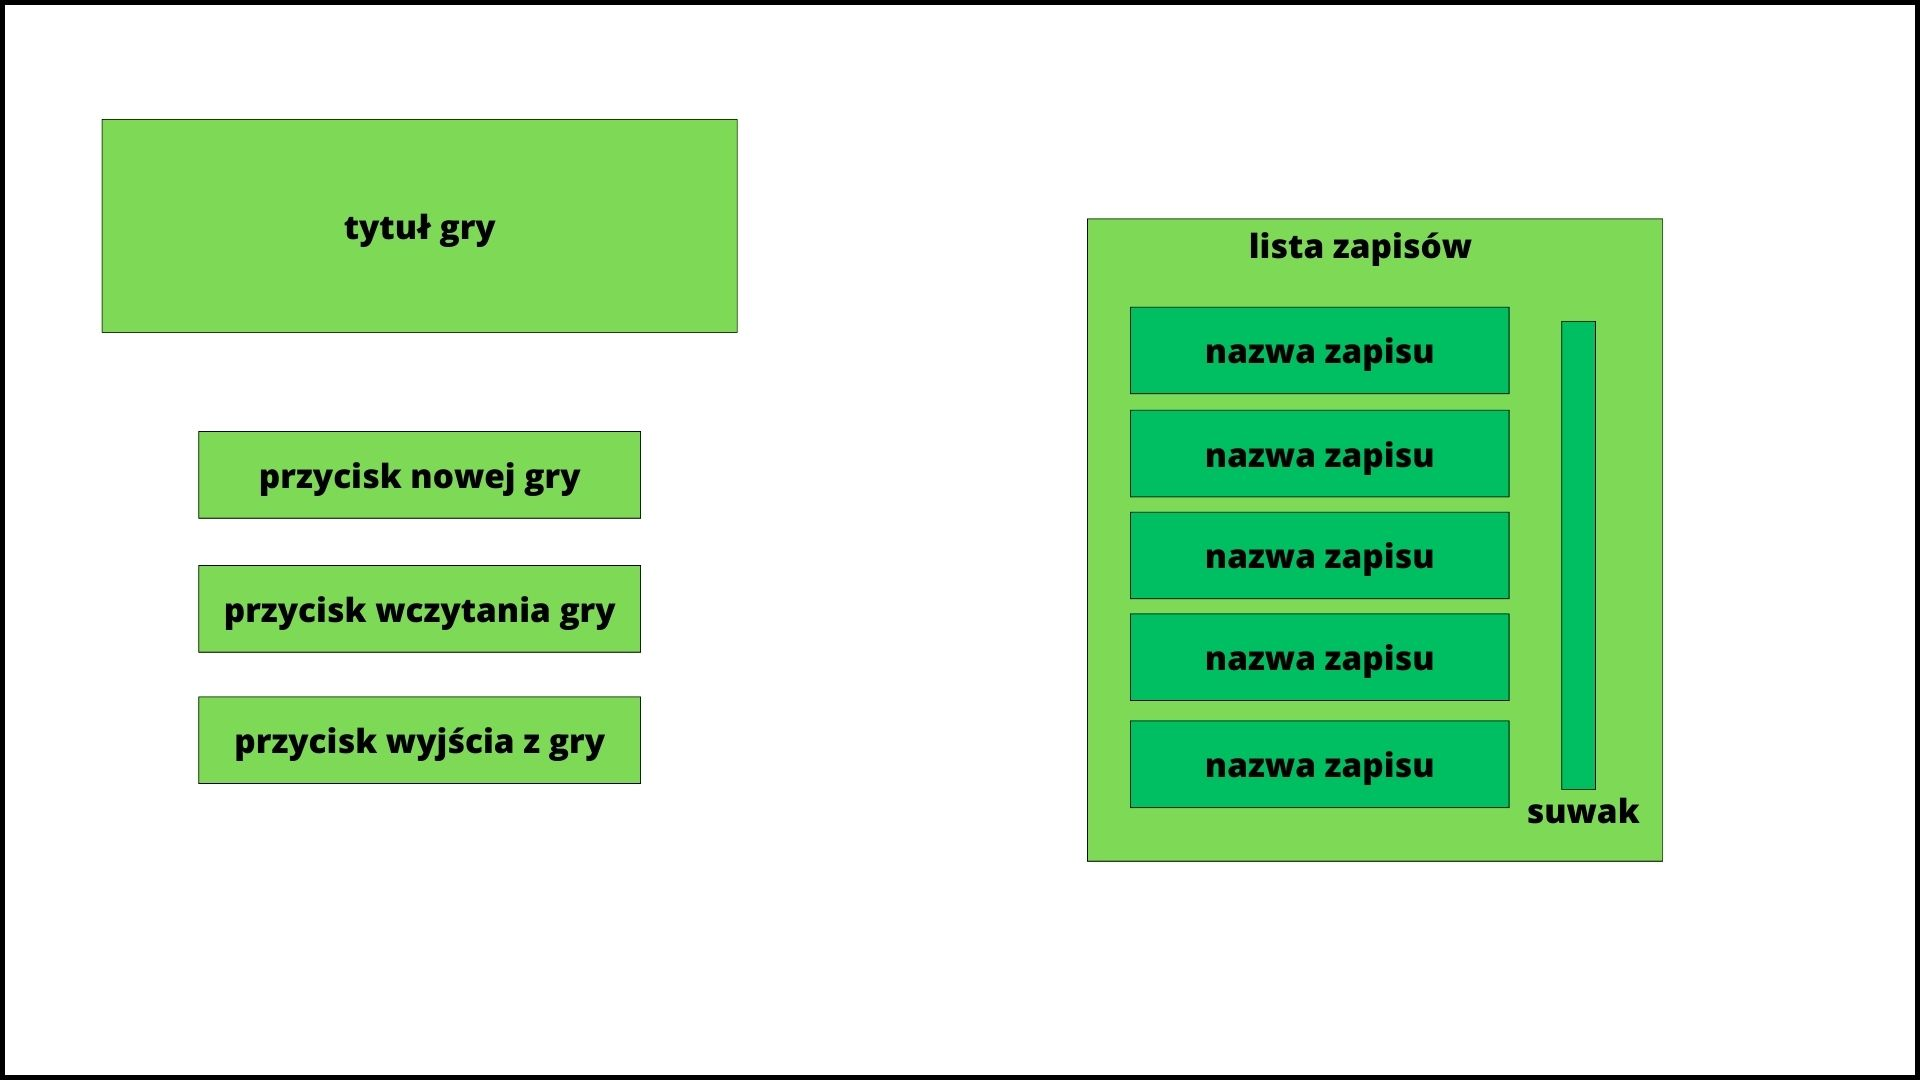
\includegraphics[width=0.8\textwidth]{images/ui/ui_prooj_menu.jpg}
    \caption{Projekt menu głównego.
    }\label{fig:compass}
\end{figure}
